\chapter{\label{ch:4-VERITASRealData} Challenges of Applying Deep Learning Event Classification Methods to Real Observations with VERITAS}
\minitoc
\begin{abstract}
    It is becoming increasingly recognised that artefacts in real IACT observations have the potential to seriously disrupt the efficacy of deep-learning-based event classifiers. This issue has so far been relatively poorly understood, and these artefacts are not modelled in simulations. In this chapter, we attempt to investigate the difficulties in performing observations with real observations from VERITAS when a deep learning event classifier is used. In contrast with previous efforts with H.E.S.S. data, we do not use tailcut image cleaning with charge data. We also explore the limitations of using a custom simulation approach as a means of mitigating real observations issues, as well as the utilisation of Bayesian optimisation (which for the first time we attempt to use against real IACT observations). After developing a pipeline for performing deep learning analysis with VERITAS data, we present the first detection of the Crab Nebula using a deep learning event classifier with a stereoscopic IACT array. We conclude that with current computational power and techniques, the complexity and cost of optimising deep learning event classifiers in this manner is significant. Whilst these methods are still promising, this limits the current practicality of these methods to current generation instruments or data from CTA.
\end{abstract}

\section{Introduction}

In this chapter, we explore potential issues with the application of CNN-based classifiers that have been trained with simulations against real low-level data from VERITAS. In contrast with Chapter \ref{ch:3-TimingInfo} we cannot use timing information with VERITAS. This is as VERITAS has a $\mathrm{\sim7\,ns}$ timing jitter in the peak time results. Therefore we concern ourselves with methods using integrated charge-only images, similar to more conventional IACT analysis. Given the results in Chapter \ref{ch:3-TimingInfo}, where we found that there was no potential for separating electron-induced events from $\gamma$-ray events, we do not include electrons in this analysis. 

Our ConvLSTM algorithms have thus far been trained entirely with simulated data. There are potentially serious issues to be considered when applying these techniques with real observations: variations in night sky background levels, disabled pixels or front end electronics, bright stars in the field of view, cloud cover and the reduction of telescope optical efficiency with age could all create biases in the CNN response. Not all of these effects are trivial to simulate. The aim of this chapter is to determine the extent to which these artefacts influence the ability of deep learning methods to detect astrophysical sources in real observations, and determine what, if any, strategies to combat this might be feasible. This problem of training deep learning models with simulated data is not unique to IACTs; training computer vision models with simulations is a problem present in many other research areas such as autonomous driving \cite{gtav} and facial recognition \cite{simgan}.

We investigate two novel approaches. The first is the application of custom Monte Carlo simulations as training data, and the second the use of Bayesian optimisation to determine model hyperparameters.

\section{A VERITAS Deep Learning Analysis Chain}
Unlike for CTA, where the complete pipeline for taking IACT event images and creating astronomical data products is still under development, VERITAS has a very stable data pipeline which has been under development since 2004. This stability is part of our motivation for utilising VERITAS for this study. As the earliest studies of deep learning analyses for IACTs only date back to 2016 \cite{feng2016}, the VERITAS pipeline was not designed for this purpose. Developing an analysis chain capable of taking real and simulated VERITAS data and producing detections using deep learning analysis was therefore a complex task. This section details the stages to this analysis, and how we developed a `bootstrap' counterpart deep learning analysis chain. We will begin by discussing the steps of performing standard IACT analysis using the \textit{Eventdisplay} package \footnote{Throughout this chapter, we adopt some conventions standard in VERITAS. The 'gammaness' quantity can interchangeably be referred to as an `isGamma score', similarly we swap ROC curves for `Signal Efficiency' curves, which are equivalent bar the x axis being inverted.}.

\subsection{\textit{Eventdisplay}}

\textit{Eventdisplay} (primarily written by Maier and Holder \cite{evdisp}) forms the basis of one of the two analysis chains used for VERITAS. It has also been used to generate IRFs for CTA. Using the root software framework \cite{root}, the \textit{Eventdisplay} pipeline can be used to generate astronomical spectra, lightcurves and skymaps from IACT data. Its main steps are:

\begin{itemize}
\item The Eventdisplay Step: This concerns low-level calibration of the VERITAS camera images (such as pedestal subtraction and flat-fielding) along with generation of Hillas parameters. This step can also be used to produce Data Storage Tape (DST) files containing calibrated event images, which are not normally stored during standard analysis, but which are required for performing deep learning analysis. This computationally intensive step is not generally stored to disk for reasons of efficiency.

\item The Mean Scaled Width (MSCW) step: This takes the image-wise Hillas parameterisations of the images from the cameras and combines them to generate the mean scaled width and length parameters for a given event. BDT event classification is also performed at this step. 

\item The Anasum Step: This takes information from the MSCW step and uses it to generate the required data for the creation of Skymaps and Spectra (in particular the directional separation of events into ON and OFF regions). 

\item The Plotting Step: This contains two root classes (VPlotAnasumHistograms and VEnergySpectrum) to plot astronomical sky significance maps and spectra.

\end{itemize}

Further details of specific elements of the analysis chain we implemented are detailed in the next two subsections.
\subsection{Disabled Pixels}
VERITAS's camera consists of standard (non-silicon) high-efficiency \cite{vercam} Hamamatsu R10560-100-20 MOD vacuum photomultipliers. They have a quantum efficiency greater than 32\%. It is unsafe to saturate these routinely, and such pixels have safeties built into them to shut the pixel down if the current in the PMT is too high (though this depends on the gain in the PMT). Particularly in the case of bright stars, this results in blocks of up to four pixels (due to the VERITAS Point Spread Function) that are classified as disabled and so don't record data in a given event window. Pixels may also be absent due to faulty electronics. Such disabled pixels are one of the prime culprits of discrepancies between real and simulated data, so we designed an interpolation strategy for the real observations that replaces the zeros in the image arrays for these pixels and interpolates based on pixel intensity values up to six pixels away in the un-mapped image.  


\subsection{Image Mapping}
The VERITAS cameras consist of 499 photomultipliers as shown in Figure \ref{fig:verc} \cite{vercam}. As the camera is not square, an appropriate geometric transformation must be applied. To do this, we use the ImageMapping classes from the CTA dl1-data-handler project \cite{dl1dh}. The analysis pipeline we have developed (see Section 2.9) writes, and can process, VERITAS data transformed in 8 different ways: axial addressing, oversampling, rebinning, nearest interpolation, bilinear interpolation, bicubic interpolation and image shifting. However, internal results from the CTA consortium have shown that the effect of the difference between these mapping methods is negligible on simulations \cite{nietopc}. So we primarily concern ourselves with oversampling for the rest of this chapter; a future study could look into this issue in further detail with this pipeline.
\begin{figure}[h]
        \begin{center}
        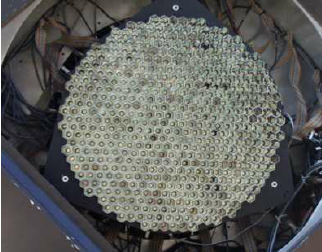
\includegraphics[width=0.6\columnwidth]{figures/verc.png}

        \caption{
                \label{fig:verc} 
                The VERITAS camera design, taken from \cite{vercam}. Note the use of Winston cones to cover the complete focal plane, needed due to the conventional photomultipliers used.
        }
        \end{center}
\end{figure}


\section{Simulations}
The first issue that we contend with in this section is choice of training dataset; which also encompasses choices regarding image cleaning and data pre-selection cuts. The training data should resemble the real observations as closely as possible, but there is a computational trade off between using run-wise simulations (which match the particular set of observations as closely as possible) and completely diffuse training data. All previous attempts at using CNN-based methods have relied upon using tailcut-cleaned images \cite{Shilon} for both the simulated training data and the real test data. We consider this to be counter-productive for background rejection \footnote{This may not be the case for directional reconstruction studies, in which CNNs appear very promising}, despite the fact this procedure simplifies the real observations problem (as it removes the need to accuracy model an entire image with for example 499 pixels vs $\sim$8). Our reasoning for considering tailcut cleaning unhelpful is that the purpose of investigating CNNs for $\gamma$/hadron separation is to utilise their sensitivity to minute features in the air shower images. These small features, such as hadronic halos \cite{model++} (Cherenkov light from the incident primary charged hadron) or subtle electromagnetic substructure would be removed by tailcut cleaning. As such, whilst using it may provide comparable results to BDTs on bright sources such as PKS 2155-304 \cite{Shilon}, using tailcut cleaning partially defeats the purpose of using CNNs for background rejection. Methods reliant upon such cleaning are unlikely to provide a sufficient increase in performance to justify the high computational cost of deep learning techniques.

Whilst there is a large amount of literature available on the problem of domain adaptation \cite{ada}, the field remains in it's relative infancy. Given the negligible performance improvement using conventional simulations with a CNN-type approach that utilise image cleaning seen in \cite{Shilon}, \cite{ParsonsOhm}, we speculate that one potential source of error with these CNN-type methods is discrepancies between these conventional simulation approach and the observational data. We speculate that one potential means of bridging this gap will be a partial run wise simulation approach in order to minimise these difference between training and test data. This is a new paradigm in $\gamma$-ray astronomy \cite{rws}, pioneered by the H.E.S.S. collaboration, and entails generating a unique simulation dataset for every run (28 minutes for H.E.S.S., 20 or 30 minutes for VERITAS) of data collection. The notable achievements of this strategy include the detection of the extension of Centaurus A by an IACT \cite{cena}. The VERITAS simulation chain is limited in its ability to reproduce as many run wise effects as H.E.S.S., though we aim to reproduce this approach as much as possible. These simulations were generated using the \textit{CORSIKA} and \textit{CARE} \cite{CARE} simulation packages. \textit{CARE} fulfils the same instrument simulation role in VERITAS as \textit{sim\_telarray} does in CTA and H.E.S.S..

\subsection{Magnetic Field Effects}
In the following subsections we will discuss specific elements of the simulations we utilised. Because of the Lorentz force, and the comparatively strong geomagnetic field at the VERITAS site \cite{kraus}, VERITAS shower images are broadened in differing directions as a function of azimuth. This magnetic field has an overall magnitude of 47 $\mu$T, but the effect of this is is dependent upon the angle between the shower and magnetic field, so only a component of this has an effect on the shower morphology.  To account for this, we match the altitude and azimuth of the simulations to the mean run values in Table \ref{table:obssummary}, with a 5 degree opening angle for both the simulated $\gamma$-rays and protons.

\subsection{Energy Thresholds}
As with all new techniques, the energy thresholds for \textit{CORSIKA} simulations that should be used when attempting to apply deep learning methods to real observations must be determined iteratively. Set the energy threshold too low, and the classifier will struggle to converge on training data (particularly for proton showers which produce relatively little Cherenkov light as a function of energy). But set it too high, and you might loose an improvement in sensitivity at low energies that CNN-type methods might bring. We concluded that using a \textit{CORSIKA} energy range of $\mathrm{100\,GeV-200\,TeV}$ for the $\gamma$-ray simulations, and $\mathrm{300\,GeV-600\,TeV}$ for the proton simulations was appropriate as a first step, but further investigations to lower this energy threshold could be performed (this was after achieving poor results with a lower energy threshold of $\mathrm{30\,GeV}$ for both protons and $\gamma$-rays). One of the issues with comparing CNNs with Hillas-parameter based methods is that for low energy events or events which only have a small number of triggered pixels in certain telescopes Hillas parameter extraction will fail. This is not the case for CNN-type methods which will attempt to classify sets of images from an event regardless of the number of triggered pixels in each telescope.

\subsection{Energy Spectrum and Event Ratios}
Throughout the work in Chapter \ref{ch:3-TimingInfo}, and through our initial investigations into real observations, we have been using simulations with power law spectra and equal ratios of events (albeit over differing energy ranges). It may be argued that this source model is overly simplistic for our purposes. Firstly, not every $\gamma$-ray source on the sky is equally bright, so the ratio of $\gamma$-ray to proton events will not be the same for every observation. Secondly, the spectra both of astrophysical gamma-ray sources and of the cosmic ray background is not a straight power law. This results in an energy dependence in the ratio of gamma-ray to proton events. Thirdly, there is a dependence on low-level trigger selection cuts, if data is only stored for events that produce a certain amount of Cherenkov light then this affects the ratio of stored $\gamma$-rays to stored protons. However, a counterargument to this is that with fewer events at a given energy the ConvLSTM will train less well; and there is a trade off to be had between training efficiency and resembling real observations closely. As such, in this chapter we attempt to balance these effects, and use the VERITAS standard -1.5 spectral index for the training data. Given the ratio of events after basic event pre-selection is approximately 1:1 for the Crab Nebula, we use this as our event ratio in our training data.

\section{Gammaness Cut Optimisation}
Gammaness ($\Gamma$) is the score given to a given event representing how closely the event resembles a $\gamma$-ray. In the \textit{Eventdisplay} framework this is a float in the range [-0.5,0.5]. Typically one discards events from the analysis which have a $\Gamma$ below a particular value, which has to be optimised for the source flux in question. 

Our 2DConvLSTM produces a vector (\textbf{x}) containing two values (one for each event class,   $\textbf{x}_1$ for $\gamma$-rays $\textbf{x}_0$ for protons). The values in this vector span the range [0,1] and must sum to 1. From this, we can construct a $\Gamma$ score through:

\begin{algorithmic}
    \IF{$argmax(\textbf{x}$)=0} 
    \STATE $\Gamma=0.5-\textbf{x}_0$
    \ELSE
    \STATE $\Gamma=\textbf{x}_1-0.5$
    \ENDIF
\end{algorithmic}
There is a question as to how meaningful this particular score is, and the role to which model uncertainty might play. We discuss the possibility for future Bayesian Neural Network analysis in Chapter \ref{ch6-Conclusions}.

For conventional BDT analysis methods, the choice of $\Gamma$ cutoff is optimised to maximise the signal-to-noise ratio for a source. However, this algorithm is known to be difficult to translate to deep learning methods, details of this issue can be found in \cite{Shilon}. For the purposes of our work in this chapter we simply pick a $\Gamma$ value of 0.2.

\section{The Crab Nebula}
The Crab Nebula was the first astrophysical $\gamma$-ray source reliably detected from the ground, in 1989 by the Whipple Observatory \cite{weekestev}. It is the remnant of a massive star that exploded in 1054AD; this explosion was recorded by Chinese observers as a `guest' star \cite{lhassocrab}. The first Whipple detection was due to a mixture of advances in Cherenkov camera technology and the advent of early Hillas analysis for background rejection. \cite{hillasparams}. Earlier `detections' largely relied upon pulsar folding methods that have since been found to be incorrect \cite{paulathesis}, partly as they were limited by available camera technology at the time. As a result, the Crab Nebula is one of the most extensively studied $\gamma$-ray objects, and has recently been found to be extended at IACT energies \cite{holler}. In 2019, it was found by the Tibet AS-$\gamma$ experiment that the Crab Nebula produced some of the highest energy photons ever detected, resulting in a 5$\sigma$ detection of the Nebula at over $\mathrm{100\,TeV}$ \cite{asgamma}. $\mathrm{1.1\,PeV}$ photons recently detected by LHASSO are also evidence of the Crab being a galactic source of PeV cosmic rays (making the Crab a so-called PeVatron) \cite{lhassocrab}. These reasons make the Crab Nebula our first analysis target, though there are a number of complications associated with this (particularly the greater number of bright stars in the camera field).

\section{Methods}
\subsection{Our Analysis Framework}
Our framework to bootstrap the \textit{Eventdisplay} analysis chain consists of three main steps:

\begin{itemize}
    \item HDF5 file dumpers to convert both simulated and real VERITAS images in .root DST files into a format suitable for deep learning. This includes image mapping and mixing of proton/$\gamma$-ray simulations as appropriate. To obtain data from the root DSTs we use the \textit{root\_numpy} \cite{rootnumpy} package.
    \item \textit{Keras} scripts to perform training and testing of the ConvLSTMs, and write test predictions for a given event to file.
    \item Scripts to take a .root file generated using the normal analysis chain and add an additional tree containing the ConvLSTM predictions in order to make spectra and skymaps.
\end{itemize}

The analysis structure for performing this is shown in Figure \ref{fig:Gettingout}, and the associated code can be found at \url{https://github.com/STSpencer/Getout}. Modifications to the \textit{Eventdisplay} code were also necessary in order to handle both the new deep learning results and the use of run-wise simulations. A significant complicating factor was matching exactly the same number of predictions with the number of events in the data .root files. This mandated testing events individually with a batch size of 1, which slowed the deep learning analysis. A future sufficiently flexible end to end CTA pipeline would avoid this step; we discuss the potential for this in Chapter \ref{ch6-Conclusions}.
\begin{figure}[h] 
        % read manual to see what [ht] means and for other possible options
        \centering 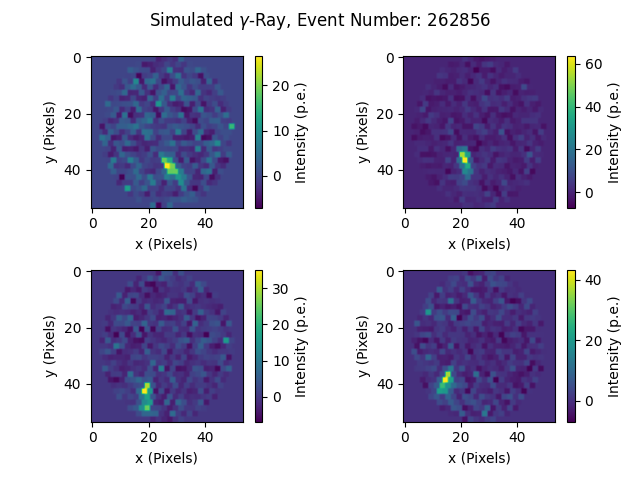
\includegraphics[width=0.8\columnwidth]{figures/sim_272_oversampling.png}

        \caption{
                \label{fig:sim} A simulated VERITAS MC $\gamma$-ray imaged using the oversampling technique. This event is shown as input to the ConvLSTM2D, without image cleaning applied.
        }
\end{figure}
\begin{figure}[h] 
        % read manual to see what [ht] means and for other possible options
        \centering 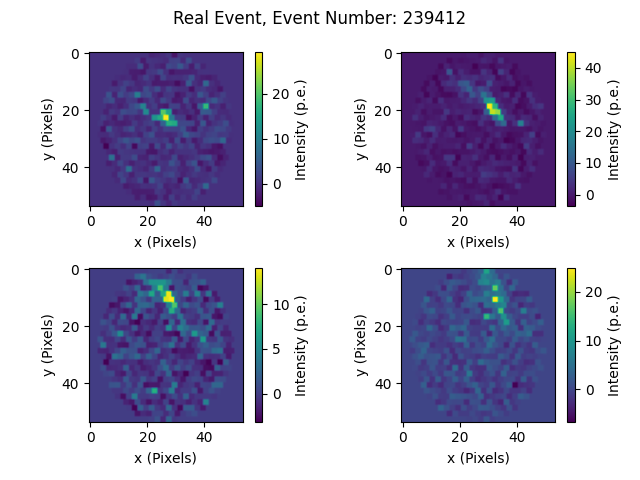
\includegraphics[width=0.8\columnwidth]{figures/realevent_303_oversampling.png}

        \caption{
                \label{fig:real} For comparison with Figure \ref{fig:sim}, a real VERITAS event from run 64080, for which there is no ground truth available. Note that the detector electronics is simulated whereas realistic NSB is not.
        }
\end{figure}
\begin{figure}[t!] 
        % read manual to see what [ht] means and for other possible options
        \centering 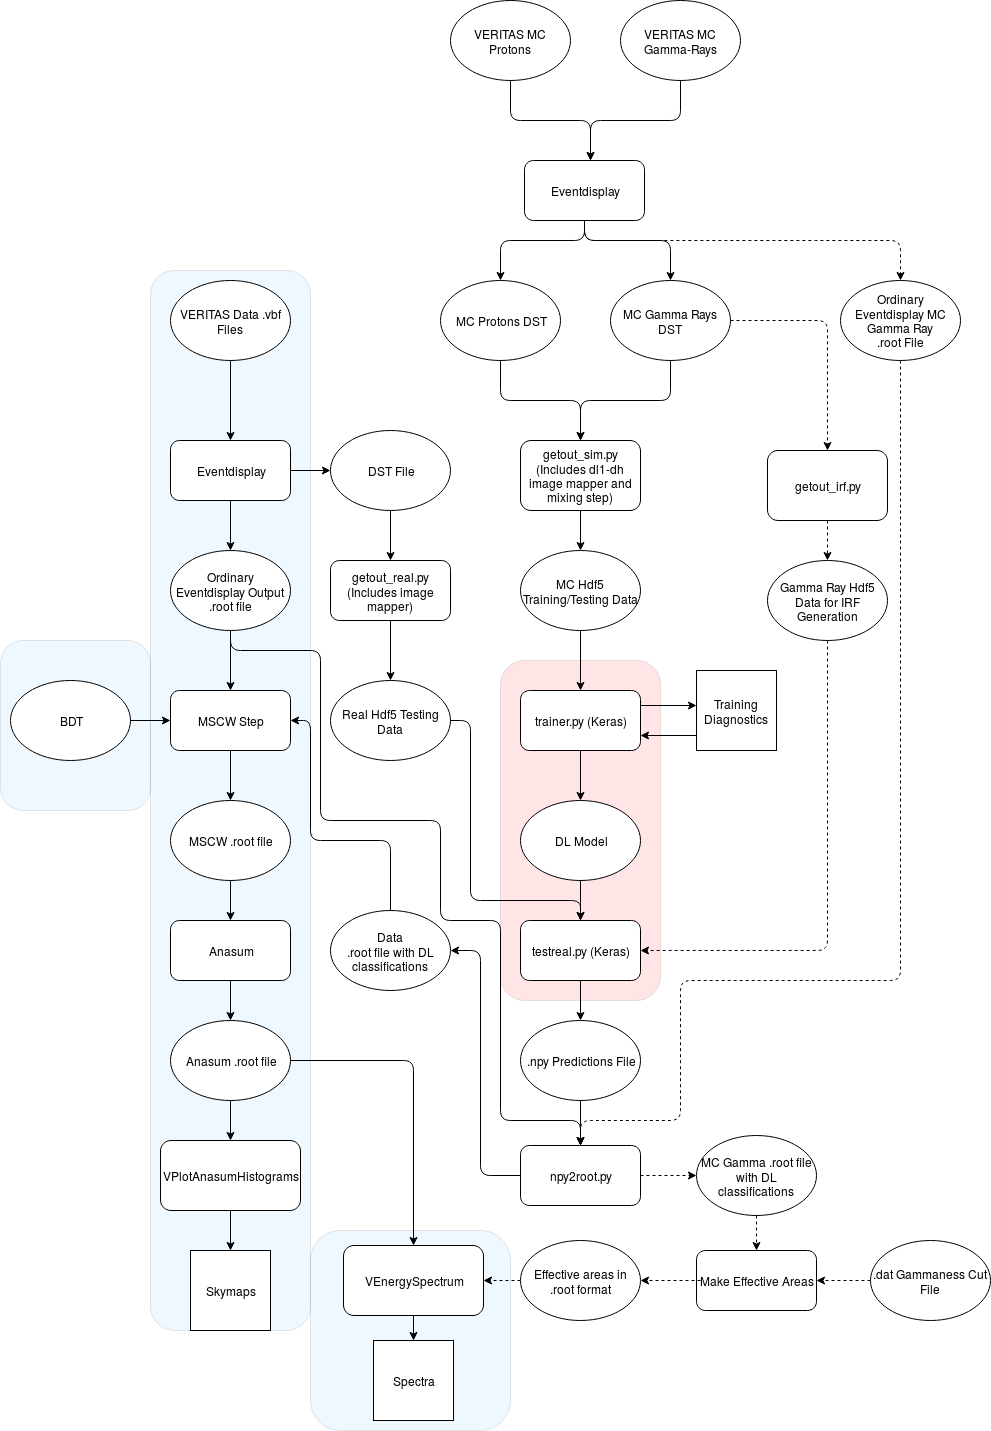
\includegraphics[width=0.83\columnwidth]{figures/Gettingout.png}

        \caption{
                \label{fig:Gettingout} The analysis pipeline I have created in order to perform CNN-based event classification using the VERITAS array. Rectangles represent analysis scripts whereas ellipses represent stored data and squares output products. In the shaded blue region is the standard Eventdisplay pipelines, and on the right is the CNN classification pipeline. The shaded red region indicates code that was run on our group's Nvidia 1080Ti GPU in Oxford, for which there are associated transfer steps in order to relay this information to the computing cluster at DESY. The dashed lines show the pipeline for creation of Effective Areas. The only step not currently implemented is the generation of spectra.
        }
\end{figure}

%This is crabrun2b
\subsection{Effective Areas}
 Effective areas represent the collection area of the IACT array as a function of energy ($E$), and are necessary to generate astrophysical spectra. Our pipeline can generate effective areas, and this gives us an idea of how well our event classifier performs as a function of energy.  They are derived from a $\Gamma$ cut value and Monte Carlo (MC) simulations of $\gamma$-rays through the formula

\begin{equation}
    A_{eff}(E,\theta,\phi)=A_0\left(\frac{\textrm{Number of }\gamma\textrm{-rays that pass event selection }(E,\theta,\phi)}{\textrm{Total number of }\gamma\textrm{-rays }(E,\theta,\phi)}\right)
\end{equation}

which includes a dependence on zenith ($\theta$) and azimuth ($\phi$) angles and a normalisation constant $A_0$. 

\subsection{Issues with the Standard VERITAS Analysis Approach and Deep Learning}
There were two main complications to performing deep learning analysis with \textit{Eventdisplay}. Firstly, VERITAS does not normally use proton air shower simulations, and instead normally operates using BDTs trained on simulated gamma-rays with real proton air shower data as background. This is for reasons of speed, and because of the difficulty of simulating hadronic EAS.  This approach is detailed in \cite{kraus}. In our case for this purpose we utilised observations of the Tycho supernova remnant (not expected to contain a significant number of $\gamma$-rays) with loose Hillas parameter cuts. Early in this investigation we found that this was not going to be a viable approach for CNN-type background rejection methods as the ConvLSTM2D classifier was sufficiently sensitive to be able to determine with 100 percent efficiency the differences between simulated gammas and real proton air showers in training data. When applied to real test data this classifier was no better than a random number generator. As such, we resorted to using proton simulations as training data, in contrast to standard VERITAS operating procedure. Pre-trained BDTs trained with a different, more standard training sample (with simulated $\gamma$-rays and real protons) are supplied with \textit{Eventdisplay}.

Secondly, the VERITAS analysis pipeline is not sufficiently flexible to support the generation of spectra from effective areas produced using our custom simulation approach. Though these effective areas themselves give us some idea of the classifier performance as a function of energy, albeit only on simulated data.

\subsection{Analysis Cuts}
One of the known issues with deep learning research for IACTs is that one needs to be wary of the effect of event pre-selection cuts. These can make it appear as if deep learning methods are performing roughly as well as conventional BDT/RF analysis. However, in such instances all the effective classification power comes from the cuts selected, and the deep learning classifier is acting as a random number generator due to the previously discussed discrepancies with simulated data. Performing harsh pre-selection cuts on training data (using either Hillas parameters or total intensity of images) will improve the AUC values obtained on simulations, but restricting ourselves to such obvious cases of $\gamma$-hadron separation again defeats the purpose of using CNN-based methods. If the only events we consider are events a BDT would easily be able to classify, then there is no potential benefit of using a CNN given their significant complexity and high computational cost. As such, we use minimal dataset cuts throughout this work. We perform no cuts on training data, and only minimal cuts on the MSCW and MSCL (to remove obviously hadronic events) as well as a necessary Theta-Squared cut of 0.008 deg$^2$ that are a default part of the \textit{Eventdisplay} analysis chain on real observations. The cuts used are described in listing \ref{verb1} in Appendix \ref{app:1-VERITASCut}.

\section{Initial Results}
\subsection{Run Summaries}
We began our investigations by selecting which data to replicate. Run 64080 was selected for our investigation due to its high degree of prior investigation and stability, and clear (category A) weather conditions. The observing conditions for this run are summarised in Table \ref{table:obssummary}.
\begin{table}[h]
    \centering
    \resizebox{0.5\textwidth}{!}{
    \begin{tabular}{c|c}
    \textbf{Run Parameter} & Value\\
    \hline
    \textbf{Run Type} & Observing\\
    \textbf{Weather} & A\\
    \textbf{Run Start} & 2012-10-13 10:52:08\\
    \textbf{Observation Mode} & Wobble\\
    \textbf{Offset (RA, DEC)} & (0,0.5)\\
    \textbf{Participating Telescopes} & T1 T2 T3 T4\\
    \textbf{Number of Events} & 543481 \\
    \textbf{Elapsed Time L3 (seconds)} & 1201.8 \\
    \textbf{Live Time L3 (seconds) } & 1013.2 (84.32\%)\\
    \textbf{Mean Trigger Rate (Hz)} & 536.3\\
    \textbf{Mean Elevation (deg)} & 78.86\\
    \textbf{Mean RA, DEC (deg)}& (83.64,22.52)\\
    \end{tabular}
    }
    \caption{Observing summary for run 64080}
    \label{table:obssummary}
\end{table}

\subsection{Effect of Custom Simulations}
Figures \ref{fig:cr2_trainlog}, \ref{fig:cr2_sigeff}, \ref{fig:cr2_hist}, \ref{fig:skysig} and \ref{fig:sig1d} show the initial results from the use of this pipeline and the custom simulations alone. The neural network was not completely optimised on simulations, scoring an 83\% test accuracy and a 0.91 AUC (good results given the lack of event selection in the simulation test data). But the initial results on the real Crab data were poor, perhaps this was to be expected given the weak cuts and lack of image cleaning used in comparison to the Shilon et al. work \cite{Shilon}. In particular, it should also be noted that most of the background rejection in these results is due to a cut on the $\theta^2$ Hillas parameter necessary to perform a reflected region analysis. Despite our initial detection being a ~$7.9\sigma$ detection of the Crab Nebula (which includes very soft cuts on the MSCW and MSCL), using the cut on the $\theta^2$, MSCW and MSCL with a random number generator for $\Gamma$ scores yields a ~$7.4\sigma$ detection. Evidence for the need for a more thorough analysis of the  uncertainty in the model predictions was demonstrated by the significance not changing if a cut on $\Gamma$ is changed from 0.2 to 0.4.
\begin{table}[h]
    \centering
    \resizebox{\textwidth}{!}{
    \begin{tabular}{c|c|c|c|c|c|c}
    \textbf{Run} & $\textbf{N}_{on}$ & $\textbf{N}_{off}$ & \textbf{Significance} & \textbf{Signal Rate} & \textbf{Error on Signal Rate} & \textbf{Background Rate} \\
    & (events)&(events) & ($\sigma$) & ($\gamma$/min) & ($\gamma$/min) &( events/min) \\
    \hline
    64080 &  175 & 89.17 &   7.3 & 4.285   &0.688 & 4.451\\
    \end{tabular}
    }
    \caption{Anasum output for custom simulations alone run.}
    \label{table:RNG}
\end{table}

\begin{figure}[ht] 
        % read manual to see what [ht] means and for other possible options
        \centering 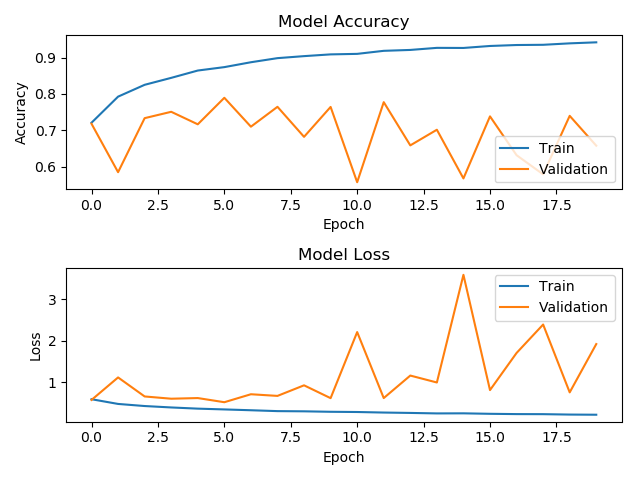
\includegraphics[width=\columnwidth]{figures/crabrun2trainlog.png}

        \caption{
                \label{fig:cr2_trainlog} The training curve for the custom simulation alone run.
        }
\end{figure}

\begin{figure}[ht] 
        % read manual to see what [ht] means and for other possible options
        \centering 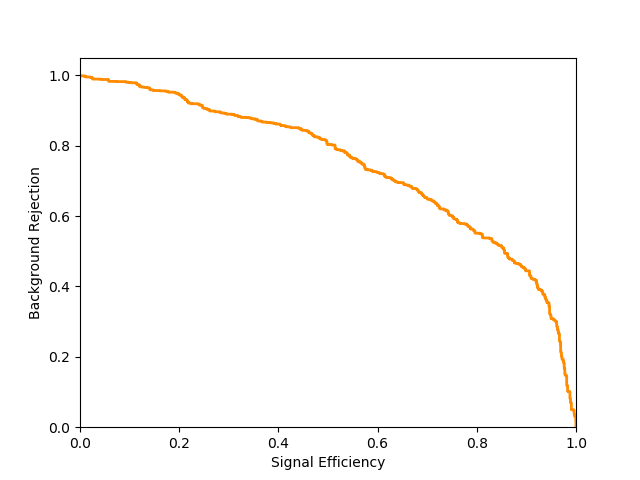
\includegraphics[width=\columnwidth]{figures/crabrun2_sigeff.png}

        \caption{
                \label{fig:cr2_sigeff} The test signal efficiency curve for the custom simulation alone run.
        }
\end{figure}

\begin{figure}[ht] 
        % read manual to see what [ht] means and for other possible options
        \centering 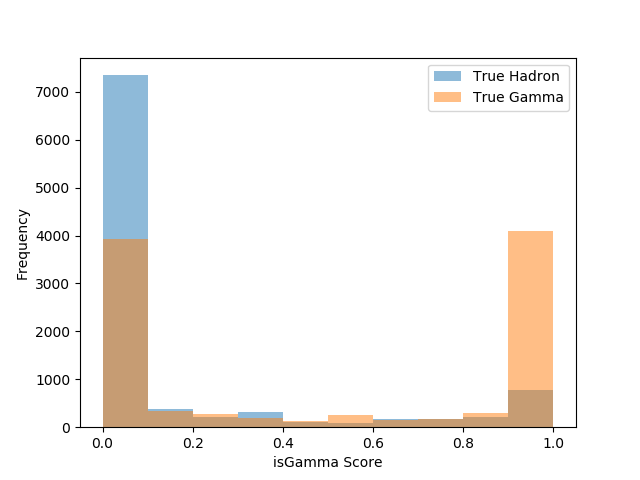
\includegraphics[width=\columnwidth]{figures/crabrun2_hist.png}

        \caption{
                \label{fig:cr2_hist} The test gammaness histogram for the custom simulation alone run. The model shows poor convergence on validation data.
        }
\end{figure}

\begin{figure}[h] 
        % read manual to see what [ht] means and for other possible options
        \centering 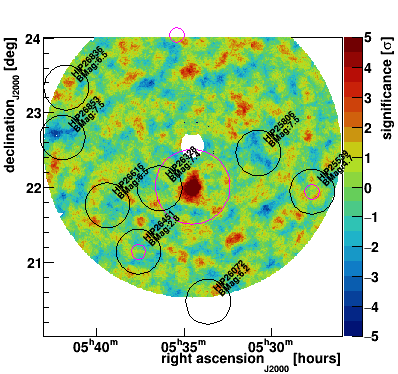
\includegraphics[width=\columnwidth]{figures/skysig.png}

        \caption{
                \label{fig:skysig} A $\gamma$-ray image of the Crab Nebula produced using the initial configuration, custom simulations and our analysis pipeline and our ConvLSTM background rejection technique along with a reflected region analysis. Regions containing bright stars recorded by the HIPPARCOS survey are also shown. Source and excluded regions are shown in purple.
        }
\end{figure}
\begin{figure}[h] 
        % read manual to see what [ht] means and for other possible options
        \centering 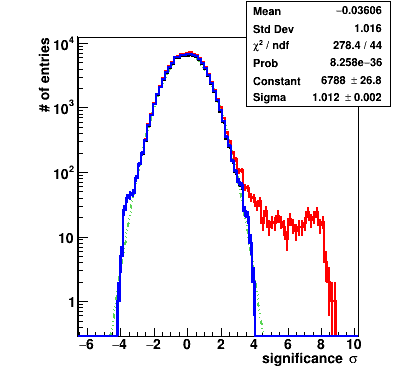
\includegraphics[width=\columnwidth]{figures/sig1d.png}

        \caption{
                \label{fig:sig1d} The 1D significance distribution including the source region (Red) and excluding it (Blue) and a Gaussian fit to the cosmic ray background (Green). Significances in IACT $\gamma$-ray astronomy are defined by \cite{LiMa}.
        }
\end{figure}
Given these results, it appears as though custom simulations (as they are achievable with VERITAS) on their own are not enough to bridge the domain gap between real IACT data and simulations. The poor, noisy performance on validation data throughout the training process is a common feature we observed in using these ConvLSTM2D methods, and is part of the reason we did not use such data in Chapter \ref{ch:3-TimingInfo}. We will find that hyperparameter selection is an important element of this, but we could also be observing a result of the small batch sizes needed to fit such models onto GPUs with finite VRAM.

\subsection{Hillas Width Analysis}
There is a legitimate question of how closely the proton simulations described earlier in this chapter match the real observations and the $\gamma$-ray simulations. If the proton simulations have major discrepancies against the real observations, and if the proton simulations are not reasonably similar to the $\gamma$-ray simulations, this may cause issues with the classifier network. As a control, we retrofit the \textit{ctapipe} Hillas extractor to extract Hillas widths from our VERITAS images for the four telescopes (CT1-4), to act on both our simulated data and the real event images (after disabled pixel interpolation).
\begin{figure}[ht] 
        % read manual to see what [ht] means and for other possible options
        \centering 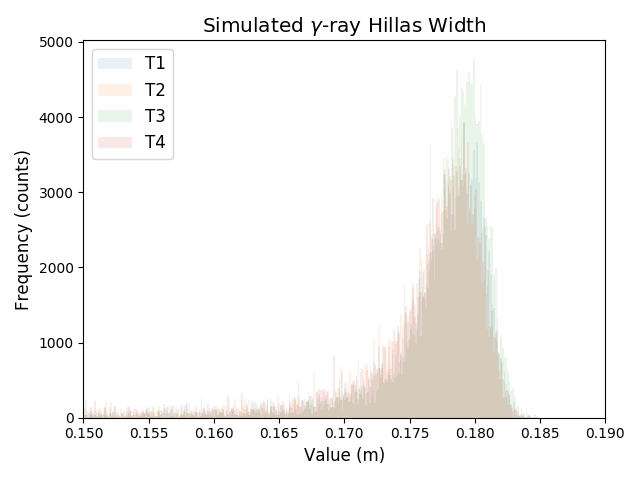
\includegraphics[width=\columnwidth]{figures/Gamma2_int.png}

        \caption{
                \label{fig:Gamma2_int} Hillas Width Distribution for the Simulated $\gamma$-rays for the four telescopes.
        }
\end{figure}
\begin{figure}[ht] 
        % read manual to see what [ht] means and for other possible options
        \centering 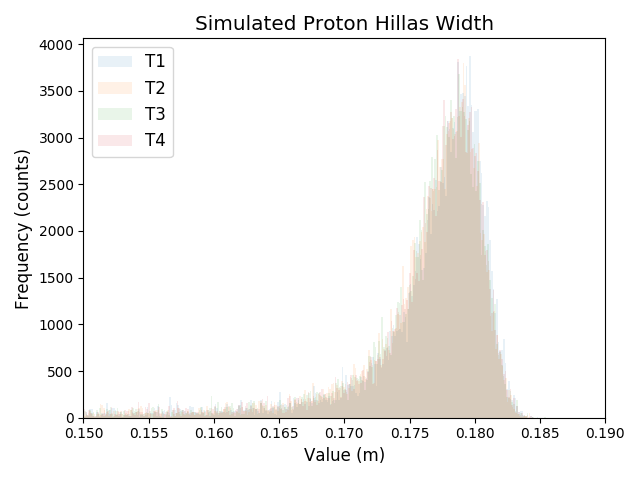
\includegraphics[width=\columnwidth]{figures/Proton2_int.png}

        \caption{
                \label{fig:Proton2_int} Hillas Width Distribution for the Simulated Protons.
        }
\end{figure}

\begin{figure}[ht] 
        % read manual to see what [ht] means and for other possible options
        \centering 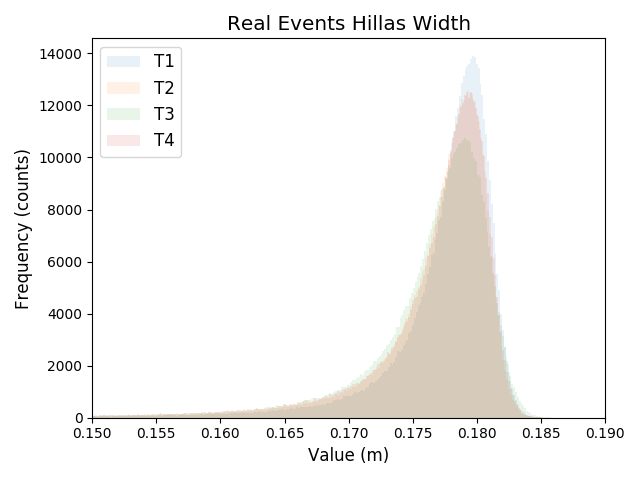
\includegraphics[width=\columnwidth]{figures/Real_int.png}

        \caption{
                \label{fig:Real_int} Hillas Width Distribution for the Real Events (Run 64080). 
        }
\end{figure}

The results from this investigation are shown in Figures \ref{fig:Gamma2_int}, \ref{fig:Proton2_int} and \ref{fig:Real_int}, and we show these results averaged by telescope and normalised such that the distributions integrate to unity in \ref{fig:telaveragedwidth}. All three width distributions are of similar shape with close peak values, suggesting our simulation choice was sound. There are more events for the real data in Figure \ref{fig:Real_int} here due to a \textit{ctapipe} feature that cuts off the analysis if the Hillas parameter extraction fails for the first telescope. The reason for the per telescope discrepancies in distributions in the real observations in Figure \ref{fig:Real_int} is because the real data contains both proton and $\gamma$-ray events; a similar per-telescope discrepancy can be seen in the simulated $\gamma$-rays in Figure \ref{fig:Gamma2_int}. The total number of training events for the ConvLSTM analysis and the real observations are unaffected by this.
\begin{figure}[ht] 
        % read manual to see what [ht] means and for other possible options
        \centering 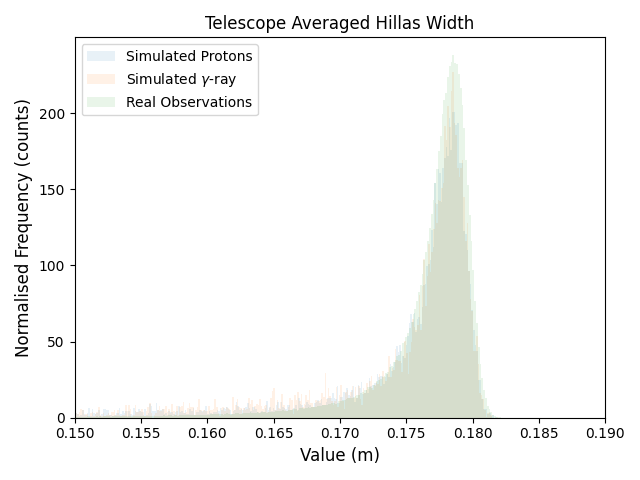
\includegraphics[width=\columnwidth]{figures/telaveragedwidth.png}

        \caption{
                \label{fig:telaveragedwidth} For ease of comparison, the telescope-averaged Hillas width distribution for the simulated proton, $\gamma$-ray and real events from Run 64080, normalised such that the distributions integrate to unity. The real observations appears to be marginally wider than the simulations, this is likely a limit of the hadronic interaction modelling in CORSIKA.
        }
\end{figure}
\subsection{Bayesian Optimisation}
Hyperparameter selection can have a significant effect on deep learning performance, so we began to consider hyperparameter optimisation, in the hope that better performance on the simulated training data might translate into increased significance on-sky. This is not guaranteed to be the case; it is entirely possible that over-optimising the classifier performance on simulated data might cause the classifier to prioritise artefacts in the simulated data not present in the real observations. Hyperparameter optimisation is broadly defined as determining $x^*$, the set of hyperparameters that maximize the objective (minimise the loss) function ($f(x)$) of a machine learning algorithm on  data $x$ \begin{equation}
    x^*=\arg \min_{x \in \chi} f(x)
\end{equation}
where $x$ is in a space $\chi$.

One of the most common approaches to hyperparameter optimisation is Bayesian optimisation, and in particular the Tree Parzen Estimator (TPE) approach \cite{bergestra} \cite{tdshyper}. Alternatives include evolutionary (designed to mimic genetic mutation) and gradient-based approaches, we briefly consider the potential for these methods in Chapter \ref{ch6-Conclusions}. One of the key advantages of this method, unlike other Bayesian optimisation approaches (such as Gaussian processes), is that it is not necessary to specify a Bayesian prior in advance of the analysis. This is well suited to deep learning analysis as the effect of the hyperparameters of a CNN are not always directly human-interpretable. Additionally, one wants the results of prior trials to inform the future searches (formally referred to as sequential model-based optimisation), which is not possible with random and grid search techniques \cite{tdshyper}. Leveraging this information, TPE optimisers have been shown to be substantially more effective than random searches on standard computer science datasets \cite{bergestra}. Where $y$ is the value of the objective function for a given set of hyperparameters $x^*$, the expected improvement $\textrm{EI}$ (which we aim to maximize at each step) is given by
\begin{equation}
    \textrm{EI}_{y^*}(x^*)=\int_{-\infty}^{y^*}(y^*-y)p(y|x^*)dy
\end{equation}
where $y^*$ is a threshold value of the objective function (below which $p(y|x^*)$ is zero), then TPE models construct a surrogate ($p(x^*|y)$) for the objective function indirectly using Bayes' rule
\begin{equation}
    p(y|x^*)=\frac{p(x^*|y)*p(y)}{p(x^*)}
\end{equation}
which is the probability of the hyperparameters given the score on the objective function \cite{tdshyper}. In turn, this surrogate is modelled as two separate distributions by TPE methods

\begin{equation}
    p(x^*|y) = \begin{cases} \textit{l}(x^*) & \mbox{, if }  y <y^* \\ \textit{g}(x^*) & \mbox{, if } y>=y^* \end{cases}
\end{equation}

where $y^*$ is the threshold value of the objective function. Using Bayes' theorem and substitution, the $\textrm{EI}$ can then be written (introducing a constant value $\gamma$) as 
\begin{equation}
    \textrm{EI}_{y^*}(x^*)=\frac{\gamma y^* \textit{l}(x^*)-\textit{l}(x^*)\int_{-\infty}^{y^*}p(y)dy}{\gamma \textit{l}(x^*)+(1-\gamma) \textit{g}(x^*)} \propto \left( \gamma +\frac{\textit{g}(x^*)}{\textit{l}(x)} (1-\gamma)\right)^{-1}
\end{equation}


The TPE approach then maximises the $\textrm{EI}$ by drawing values from $\textit{l}(x^*)$, and maximizing the ratio $\textit{l}(x^*)/\textit{g}(x^*)$, which in term maximises the $\textrm{EI}$ \cite{tdshyper}. In practice, the fact that the surrogate is not exactly the objective may mean that the hyperparameter choice offers no improvement in the objective. Therefore the surrogate function needs to be updated, and the use of a distribution $\textit{l}(x^*)$ helps to balance the trade-off between exploration and exploitation. In practical terms, this can reasonably be thought of as performing gradient descent over hyperparameter values, with the loss function as the quantity being optimised.

\subsection{Initial Optimisation Efforts}

To investigate the potential of Bayesian optimisation, we utilized the \textit{Hyperas} \cite{hyperas} \textit{Keras} wrapper around \textit{Hyperopt} \cite{hyperopt}. This is one of the most commonly-used Python packages for performing TPE analysis. However, given that this approach requires (at least partially) training a classifier for every point in hyperparameter space explored, this process is orders of magnitude more computationally costly than simply training a single deep learning classifier with a single hyperparameter configuration. It was also not immediately clear what the best approach to take with these methods given realistically finite compute power and time. There is a trade-off between the number of epochs to train a model for each point in hyperparameter space, the amount of data used for training and the number and range of hyperparameter space points probed. The optimal configuration for this was not known at the starting point of this research. But in practice, VRAM constraints limit the maximum possible range of hyperparameter values probed. Extending this range too far, for example in terms of number of layers, will eventually exhaust finite VRAM and cause crashes.

\begin{figure}[] 
        % read manual to see what [ht] means and for other possible options
        \centering 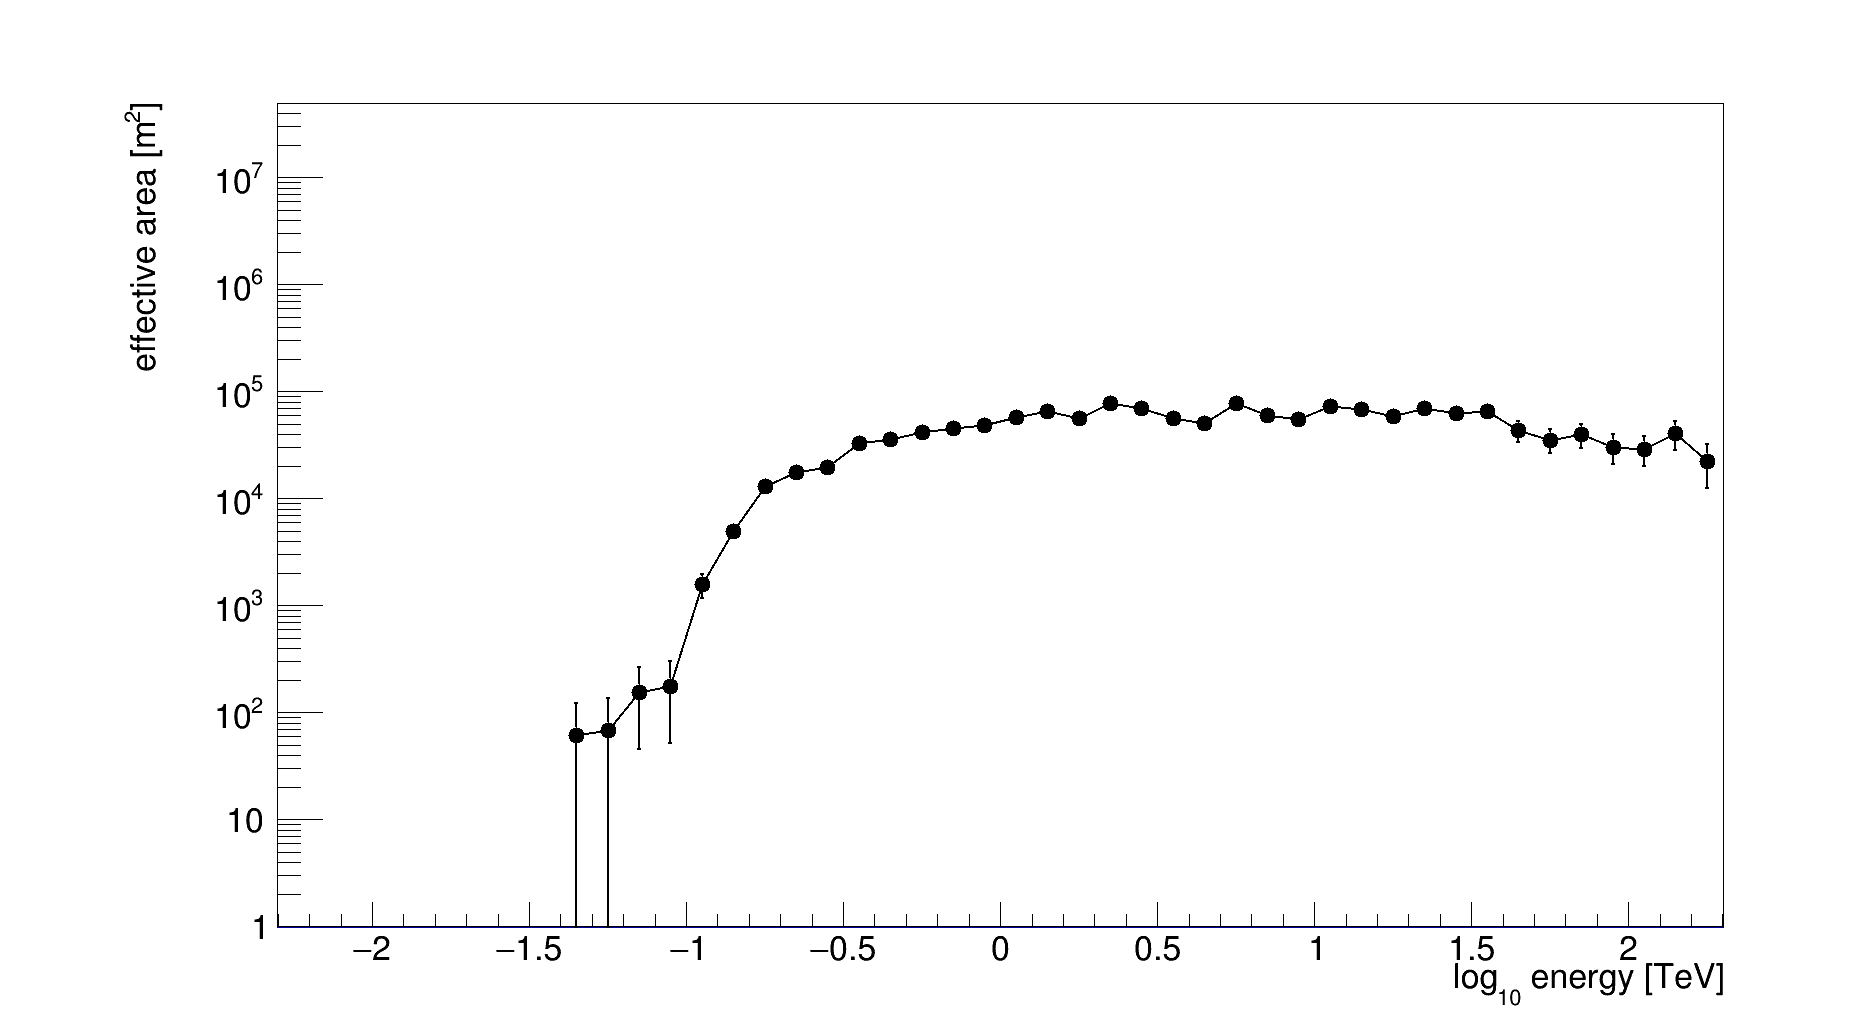
\includegraphics[width=\columnwidth]{figures/EFF.png}

        \caption{
                \label{fig:EFF} Effective area of VERITAS as a function of energy, made using our analysis pipeline and the opt4 configuration. This shows performance broadly similar to BDTs on simulations, see for comparison \cite{vereff}. However, it does not show a substantial improvement. This could possibly be an effect of the custom simulation approach we use, or as an effect of non-uniform posterior distributions on the $\Gamma$ scores from the ConvLSTM. The parameters for this are as follows: Zenith angle $10^{\circ}$, wobble offset=$0.5^{\circ}$, $\gamma$-ray spectral index=-1.5, noise level=250Hz. 
        }
\end{figure}
The initial optimisation efforts revolved around training a ConvLSTM2D classifier for a single epoch on a comparatively small number of events ($\sim$19574 simulated events) on a single GPU, using performance on a similarly small amount of validation data as a metric. The hyperparameter space for this optimisation is shown in Table \ref{table:runsopt4}, where we use hyperopt convention to define the hyperparameter space. This means Choice() represents optimising a discrete choice between a finite number of options (this can include binary selection such as the inclusion of layers, as well as selection between two dimensional objects like filter sizes) and Uniform() means the value can take any float value in a given range. The aim was to find the best `starting position' for the training. The network configuration generated following the initial hyperopt run was then trained for 100 epochs with the complete training dataset (235174 events in total). This resulted in the `opt4' configuration presented here, yielding performance superior to random number generation on the real observations. This detection represents the first time the Crab nebula has been detected with an IACT array using a stereoscopic deep-learning-based event classification method, and was the first deep-learning-based detection of an astrophysical $\gamma$-ray source not to rely upon image cleaning.

\begin{table}[ht]
    \centering
    \resizebox{\textwidth}{!}{
    \begin{tabular}{ccc|c|c|c}
    \textbf{Block} & \textbf{Layer} & \textbf{Parameter} & \textbf{Potential Values}& \textbf{Optimal Value Diffuse Source} \\
    \hline
    \hline
    \textbf{Block 1} & ConvLSTM2D & Number of Filters & Choice(10,20,30,40) &  10 \\
                     &            & Kernel Size & Choice((2,2),(3, 3),(4,4),(5,5)) & (4,4) \\
                     &            & Kernel L2 Regularizer Rate & Uniform(0,1) & 0.0797 \\
                     &            & Dropout Rate & Uniform(0,1) &  0.0361 \\
                     &            & Recurrent Dropout Rate & Uniform(0,1) & 0.382 \\
    \hline
    \textbf{Block 2} & ConvLSTM2D & Number of Filters & Choice(10,20,30,40) & 10 \\
                     &            & Kernel Size & Choice((2,2),(3, 3),(4,4),(5,5)) &  (2,2) \\
                     &            & Kernel L2 Regularizer Rate & Uniform(0,1) & 0.576 \\
                     &            & Dropout Rate & Uniform(0,1) & 0.371 \\
                     &            & Recurrent Dropout Rate & Uniform(0,1) & 0.510 \\
    \hline
    \textbf{Block 3} & ConvLSTM2D & Number of Filters & Choice(10,20,30,40) & 40 \\
                     &            & Kernel Size & Choice((2,2),(3, 3),(4,4),(5,5) & (2,2) \\
                     &            & Dropout Rate & Uniform(0,1) & 0.0 \\
                     &            & Recurrent Dropout Rate & Uniform(0,1) & 0.1 \\
    \hline
    \textbf{Block 4} &.           & Include Block & Choice(Yes,No)                      & Yes \\
                     & ConvLSTM2D & Number of Filters & Choice(10,20,30,40) &  30 \\
                     &            & Kernel Size & Choice((2,2),(3, 3),(4,4),(5,5))  & (5,5) \\
                     &            & Dropout Rate & Uniform(0,1) &  0.5056 &\\
    \hline
    \textbf{Block 5} & GlobalAveragePooling3D &  - & - &- \\
    \hline
    \textbf{Block 7} & Dense      & Number of Units & Choice(10,50,100,200) & 100 \\
    \hline
    \textbf{Block 8} & Dense      & - & - & - \\


    \end{tabular}
    }
    \caption{Summary of hyperparameter space and selected configuration for the initial single core optimisation that produced the opt4 configuration.}
    \label{table:runsopt4}
\end{table}
\begin{table}[h]
    \centering
    \resizebox{\textwidth}{!}{
    \begin{tabular}{c|c|c|c|c|c|c}
    \textbf{Run} & $\textbf{N}_{on}$ & $\textbf{N}_{off}$ & \textbf{Significance} & \textbf{Signal Rate} & \textbf{Error on Signal Rate} & \textbf{Background Rate} \\
    & (events) & (events) & ($\sigma$) & ($\gamma$/min) & ($\gamma$/min) & (events/min) \\
    \hline
    64080 &  573 & 280.17 & 13.9 & 14.617  & 1.243 & 13.985\\
    \end{tabular}
    }
    \caption{Anasum output for the opt4 run, without applying a strenuous multiplicity cut.}
    \label{table:opt4}
\end{table}

This significance of this detection is a mild function of multiplicity, the significance can reach $\mathrm{16.1\,\sigma}$ if a telescope multiplicity cut of 4 is imposed, this is a result of the signal-to-noise ratio being higher for such events. The standard VERITAS analysis, reliant upon BDTs, achieves a $\mathrm{22\,\sigma}$ detection on the same data without this strong multiplicity cut, although it is trained with a different dataset so the comparison is imperfect \footnote{Details of this analysis can be found at \url{https://veritas.sao.arizona.edu/wiki/index.php/Eventdisplay_Manual:_event_display}; but note that this is a VERITAS internal site only accessible from VERITAS member institutes.}.

\begin{figure}[h] 
        % read manual to see what [ht] means and for other possible options
        \centering 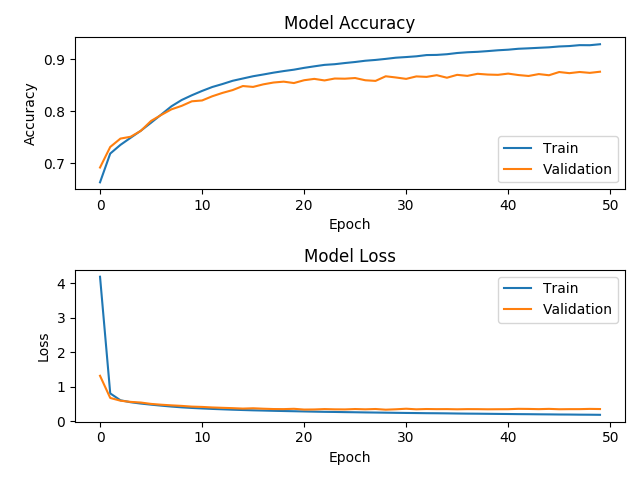
\includegraphics[width=\columnwidth]{figures/crabrun2opt4trainlog.png}

        \caption{
                \label{fig:opt4_trainlog} The training curve for the opt4 run.
        }
\end{figure}

Curiously the validation data training curve appears to converge in this one specific instance, but it is unclear if this relates to the ConvLSTM2D classifier learning meaningful features in the simulated images or if this is simply a coincidence. 

\begin{figure}[ht] 
        % read manual to see what [ht] means and for other possible options
        \centering 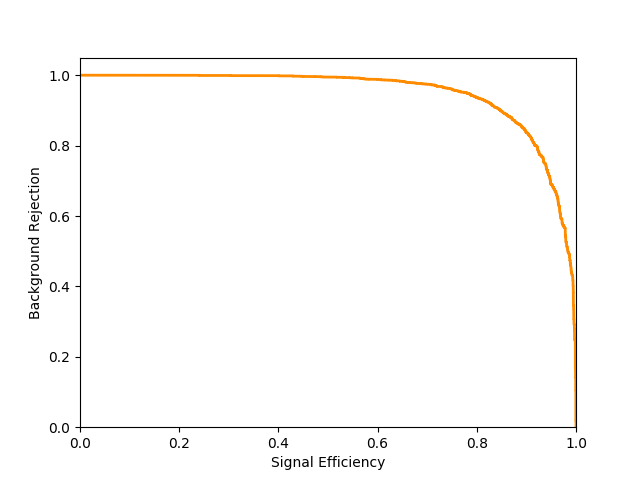
\includegraphics[width=\columnwidth]{figures/crabrun2opt4_sigeff.png}

        \caption{
                \label{fig:opt4_sigeff} The test signal efficiency curve for the opt4 run.
        }
\end{figure}

\begin{figure}[ht] 
        % read manual to see what [ht] means and for other possible options
        \centering 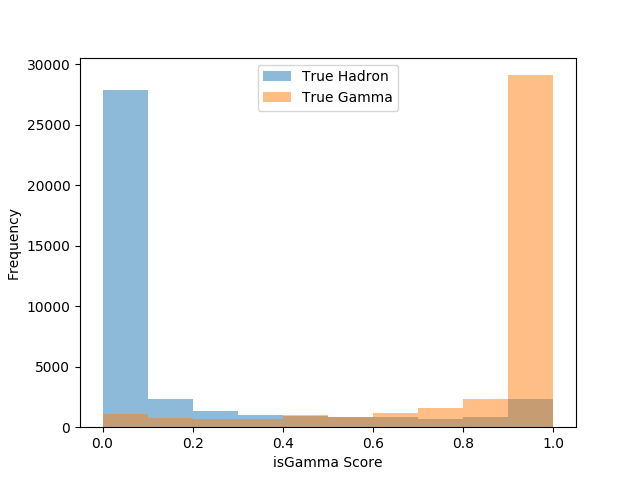
\includegraphics[width=\columnwidth]{figures/crabrun2opt4_hist.png}

        \caption{
                \label{fig:opt4_hist} The test gammaness histogram for the opt4 run.
        }
\end{figure}
\begin{figure}[ht] 
        % read manual to see what [ht] means and for other possible options
        \centering 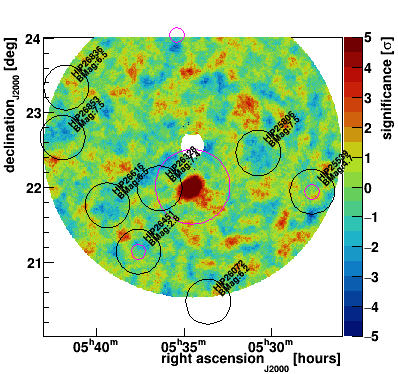
\includegraphics[width=\columnwidth]{figures/opt4_skysig.png}

        \caption{
                \label{fig:opt4_skysig} The sky significance for the 'opt4' configuration on run 64080.
        }
\end{figure}
\begin{figure}[ht] 
        % read manual to see what [ht] means and for other possible options
        \centering 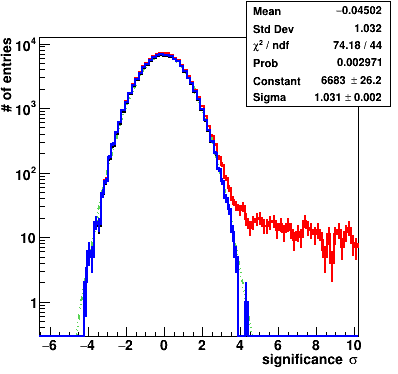
\includegraphics[width=\columnwidth]{figures/opt4_sig.png}

        \caption{
                \label{fig:opt4_sig1D} The 1D significance for the `opt4' configuration on run 64080.
        }
\end{figure}

\section{Parallelised Optimisation Attempts}
\subsection{Optimisation Configurations and Results}
Following our initial success with Bayesian optimisation, we ran extensive further investigations with improved computational power in order to test the performance limit of this new technique. The next three figures and three tables show three attempts to perform Bayesian optimisation using \textit{hyperas} in parallel using the recently upgraded \textit{glamdring} cluster. Four of the machines had two NVidia 2080Tis attached, the final had only one. The machines with multiple GPUs made use of Tensorflow's \textit{MirroredStrategy} approach, so the optimisation worker effectively saw a single GPU with double the VRAM of a 2080Ti. We'll refer to these three optimisation attempts as attempt A, attempt B and attempt C. After each optimisation attempt the best performing model was trained with the complete dataset for more epochs, similar to the earlier strategy on the single GPU. In all attempts, a unique configuration database was created, with each point in hyperparameter space being allocated a unique working directory. To operate, the optimiser consisted of a head process working on the \textit{glamdring} login node to determine hyperparameter point selection, and up to 5 worker processes on the \textit{glamdring} GPU nodes. Progress was checkpointed such that there were no information losses if a worker process failed. The classifier trained on a certain subset of training data for a certain number of epochs for each hyperparameter configuration, and the accuracy on test data after this training was used as the metric. Each of these test scores is shown as a blue cross in Figures \ref{fig:convplot_testfolders3} \ref{fig:convplot_febtry} and \ref{fig:convplot_longmoredata} , running averages and moving averages (over the maximum 4 parallel systems, each with 2 GPUs) are also shown. As individual iterations of the optimisation have some degree of randomness in order to explore the space, the only evidence of the process converging is contained within in these averages. Attempt A had a similar hyperparameter space to the initial single core optimisation run that produced the opt4 configuration, albeit using a greater number of training epochs per hyperparameter point. This hyperparameter space was increased for the subsequent attempts B and C. It should be noted that in particular optimisation attempt C, our final attempt to generate a configuration superior to the opt4 result, was extremely computationally intensive (representing the results of around 5800 GPU hours of compute time).

\begin{table}[ht]
    \centering
    \resizebox{\textwidth}{!}{
    \begin{tabular}{c|c|c|c}
    \textbf{Attempt} & \textbf{A} & \textbf{B} & \textbf{C} \\
    \hline
    \textbf{No. Training Events}                       & 39148 & 19574 & 117574 \\
    \textbf{No. Test Events}                           & 39200 & 19600 & 39200 \\
    \textbf{Epochs Training per Hyperparameter Point}  & 5     & 1     & 25 \\
    \textbf{No. Hyperparameter Points Sampled}         & 2000  & 1000  & 500 \\
    \textbf{Best Test Accuracy (\%)}                   & 77.36 & 75.9  & 86.4 \\
    \end{tabular}
    }
    \caption{Summary of parallelised optimisation runs and the amount of data used for each. Values presented here represent the number of training events, test events, and test performance for the training and evaluation during the Bayesian optimisation process. The best performing models from each optimisation run were then trained and tested again with the complete dataset for more epochs before being applied to the real observations.}
    \label{table:optsum}
\end{table}

\begin{table}[ht]
    \centering
    \resizebox{\textwidth}{!}{
    \begin{tabular}{ccc|c|c|c|c}
    \textbf{Block} & \textbf{Layer} & \textbf{Parameter} & \textbf{Potential Values}& \textbf{Optimal Value Attempt A}& \textbf{Optimal Value Attempt B} \\
    \hline
    \hline
    \textbf{Block 1} & ConvLSTM2D & Number of Filters & Choice(10,20,30,40) &  20 & 10\\
                     &            & Kernel Size & Choice((2,2),(3, 3),(4,4),(5,5)) & (4,4)& (4,4) \\
                     &            & Kernel L2 Regularizer Rate & Uniform(0,1) & 0.402 & 0.404 \\
                     &            & Dropout Rate & Uniform(0,1) &  0.462 & 0.536\\
                     &            & Recurrent Dropout Rate & Uniform(0,1) & 0.552& 0.353\\
    \hline
    \textbf{Block 2} & ConvLSTM2D & Number of Filters & Choice(10,20,30,40) & 10& 20\\
                     &            & Kernel Size & Choice((2,2),(3, 3),(4,4),(5,5)) &  (2,2)& (4,4)\\
                     &            & Kernel L2 Regularizer Rate & Uniform(0,1) & 0.234& 0.796\\
                     &            & Dropout Rate & Uniform(0,1) & 0.774& 0.563\\
                     &            & Recurrent Dropout Rate & Uniform(0,1) & 0.000& 0.116\\
    \hline
    \textbf{Block 3} & ConvLSTM2D & Number of Filters & Choice(10,20,30,40) & 30& 30\\
                     &            & Kernel Size & Choice((2,2),(3, 3),(4,4),(5,5) & (2,2)& (4,4) \\
                     &            & Dropout Rate & Uniform(0,1) & 0.444& 0.105\\
    \hline
    \textbf{Block 4} &.           & Include Block & Choice(Yes,No)                      & Yes& Yes \\
                     & ConvLSTM2D & Number of Filters & Choice(10,20,30,40) &  40& 30\\
                     &            & Kernel Size & Choice((2,2),(3, 3),(4,4),(5,5))  & (5,5)& (5,5)\\
                     &            & Dropout Rate & Uniform(0,1) &  0.720 & 0.652\\
    \hline
    \textbf{Block 5} & GlobalAveragePooling3D &  - & - &- &-\\
    \hline
    \textbf{Block 7} & Dense      & Number of Units & Choice(10,50,100,200) & 10 & 100\\
    \hline
    \textbf{Block 8} & Dense      & - & - & - \\


    \end{tabular}
    }
    \caption{Summary of hyperparameter space and selected configuration for the initial parallelised optimisation runs, attempts A and B.}
    \label{table:runsAB}
\end{table}

\begin{table}[ht]
    \centering
    \resizebox{\textwidth}{!}{
    \begin{tabular}{ccc|c|c}
    \textbf{Block} & \textbf{Layer} & \textbf{Parameter} & \textbf{Potential Values} & \textbf{Optimal Value Attempt C} \\
    \hline
    \hline
    \textbf{Block 1} & ConvLSTM2D & Number of Filters & Choice(10,20,30,40,50,60) &  10 \\
                     &            & Kernel Size & Choice((2,2),(3, 3),(4,4),(5,5),(6,6),(7,7)) & (4,4) \\
                     &            & Kernel L2 Regularizer Rate & Uniform(0,1) & 0.366 \\
                     &            & Dropout Rate & Uniform(0,1)  & 0.414 \\
                     &            & Recurrent Dropout Rate & Uniform(0,1) & 0.107 \\
    \hline
    \textbf{Block 2} & ConvLSTM2D & Number of Filters & Choice(10,20,30,40,50,60) & 10 \\
                     &            & Kernel Size & Choice((2,2),(3, 3),(4,4),(5,5),(6,6),(7,7)) &  (2,2) \\
                     &            & Kernel L2 Regularizer Rate & Uniform(0,1) & 0.167 \\
                     &            & Dropout Rate & Uniform(0,1) & 0.863 \\
                     &            & Recurrent Dropout Rate & Uniform(0,1) & 0.321 \\
    \hline
    \textbf{Block 3} & ConvLSTM2D & Number of Filters & Choice(10,20,30,40,50,60) & 40 \\
                     &            & Kernel Size & Choice((2,2),(3, 3),(4,4),(5,5),(6,6),(7,7)) & (2,2) \\
                     &            & Kernel L2 Regularizer Rate & Uniform(0,1) & 0.219 \\
                     &            & Dropout Rate & Uniform(0,1) & 0.287 \\
                     &            & Recurrent Dropout Rate & Uniform(0,1) & 0.697 \\
    \hline
    \textbf{Block 4} & ConvLSTM2D & Number of Filters & Choice(10,20,30,40,50,60) &  30 \\
                     &            & Kernel Size & Choice((2,2),(3, 3),(4,4),(5,5),(6,6),(7,7))  & (3,3) \\
                     &            & Dropout Rate & Uniform(0,1) &  0.483 \\
    \hline
    \textbf{Block 5} &            & Include Block & Choice(Yes, No)                     & Yes \\
                     & ConvLSTM2D & Number of Filters & Choice(10,20,30,40,50,60)  & 30 \\
                     &            & Kernel Size & Choice((2,2),(3, 3),(4,4),(5,5),(6,6),(7,7))  & (3,3) \\
                     &            & Dropout Rate & Uniform(0,1) &  0.020 \\
    \hline
    \textbf{Block 6} &            & Include Block & Choice(Yes, No)                     & Yes \\
                     & ConvLSTM2D & Number of Filters & Choice(10,20,30,40,50,60) &  30 \\
                     &            & Kernel Size & Choice((2,2),(3, 3),(4,4),(5,5),(6,6),(7,7))  & (3,3) \\
                     &            & Dropout Rate & Uniform(0,1) & 0.553 \\
    \hline
    \textbf{Block 5} & GlobalAveragePooling3D &  - & - &- \\
    \hline
    \textbf{Block 6} &            & Include Block & Choice(Yes, No)                     &  Yes \\
                     & Dense      & Number of Units & Choice(10,50,100,200) & 10 \\
                     &            & Dropout Rate & Uniform(0,1) & 0.190 \\
    \hline
    \textbf{Block 7} &            & Include Block & Choice(Yes, No)                     &  Yes \\
                     & Dense      & Number of Units & Choice(10,50,100,200) & 200 \\
                     &            & Dropout Rate & Uniform(0,1) & 0.743 \\
    \hline
    \textbf{Block 8} &            & Include Block & Choice(Yes, No)                     &  Yes \\
                     & Dense      & Number of Units & Choice(10,50,100,200) & 200 \\
                     &            & Dropout Rate & Uniform(0,1) & 0.107 \\
    \hline
    \textbf{Block 9} & Dense      &  - & - \\




    \end{tabular}
    }
    \caption{Summary of hyperparameter space and selected configuration for the final parallelised optimisation run, attempt C.}
    \label{table:runsC}
\end{table}

\begin{figure}[h] 
        % read manual to see what [ht] means and for other possible options
        \centering 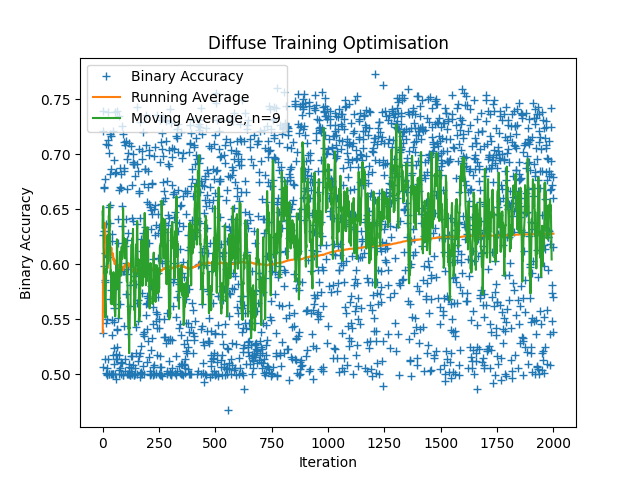
\includegraphics[width=\columnwidth]{figures/convplot_testfolders3.png}

        \caption{
                \label{fig:convplot_testfolders3} Final test accuracies after  training optimisation for longer Bayesian optimisation run attempt A.
        }
\end{figure}
\begin{figure}[h] 
        % read manual to see what [ht] means and for other possible options
        \centering 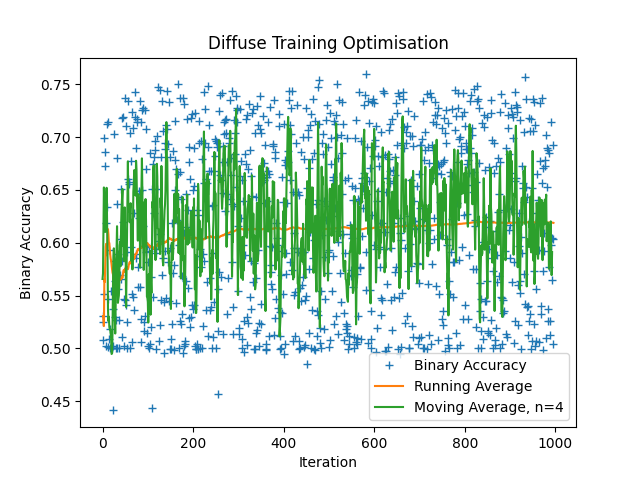
\includegraphics[width=\columnwidth]{figures/convplot_febtry.png}

        \caption{
                \label{fig:convplot_febtry} Final test accuracies after training optimisation for longer Bayesian optimisation run attempt B.
        }
\end{figure}

\begin{figure}[h] 
        % read manual to see what [ht] means and for other possible options
        \centering 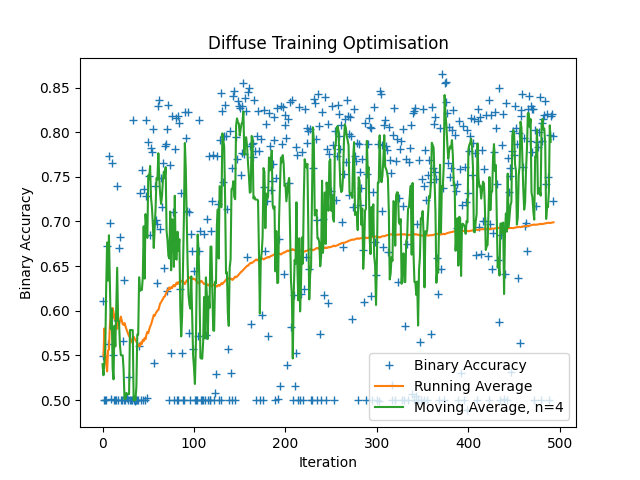
\includegraphics[width=\columnwidth]{figures/convplot_longmoredata.png}

        \caption{
                \label{fig:convplot_longmoredata} Final test accuracies after training optimisation for Bayesian optimisation attempt C.
        }
\end{figure}

Final simulated data training curves and signal efficiency curves for the best model configuration for optimisation attempt C, trained with the complete dataset are shown in Figures \ref{fig:6vimrcb1485481664_trainlog} and Figure \ref{fig:6vimrcb1485481664_sigeff} for completeness. Whilst none of these attempts generated a model superior to the opt4 configuration, this final optimisation run C is of interest as the running average shows evidence of convergence. This has not often seen with TPE methods, and this is a known issue them \cite{autosklearn}. Notably this is the first attempt at Bayesian optimisation with IACT data to ever see evidence of convergence, let alone with a stereoscopic array \cite{nietopc}. This is likely a result of the large number of epochs, the large amount of data used, and the long period the optimiser was left to run. This combined with the fact we did not achieve performance superior to the opt4 run suggests that the opt4 configuration represents the current limit of what is technically possible with deep learning event classifiers, with this configuration of simulations and cuts. Given that we observed improved performance on-sky when the classifier achieved optimal performance on simulated training data, if there is a point at which the deep learning classifier becomes `over-familiar' with the simulated data to the extent that performance with real observations is reduced, we have yet to reach it.

\begin{figure}[h] 
        % read manual to see what [ht] means and for other possible options
        \centering 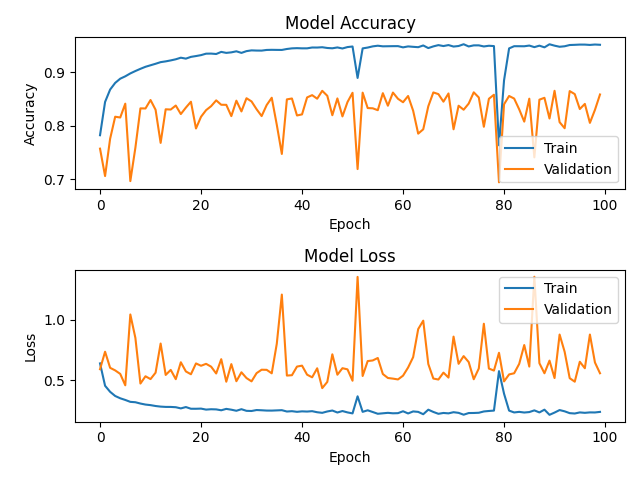
\includegraphics[width=\columnwidth]{figures/6vimrcb1485481664trainlog.png}

        \caption{
                \label{fig:6vimrcb1485481664_trainlog} Training accuracy curve for the best performing model from optimisation attempt C, trained for 100 epochs with the complete dataset.
        }
\end{figure}

\begin{figure}[h] 
        % read manual to see what [ht] means and for other possible options
        \centering 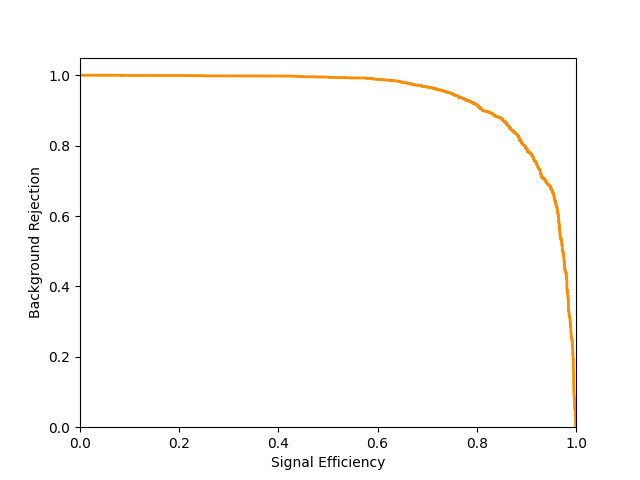
\includegraphics[width=\columnwidth]{figures/6vimrcb1485481664_sigeff.png}

        \caption{Test signal efficiency curve for the best performing model from optimisation attempt C, trained for 100 epochs with the complete dataset.
                \label{fig:6vimrcb1485481664_sigeff} 
        }
\end{figure}


\section{Conclusion}
In this chapter, we have demonstrated a deep learning pipeline capable of use with the VERITAS telescopes, and showed that a combination of ConvLSTM2D classifiers, custom simulations and Bayesian optimisation can yield a definite detection of the Crab Nebula. The is the first detection with an IACT array using such methods that did not require conventional tailcut cleaning. However, there are significant issues with this approach that limit its current efficacy for CTA that require further detailed study. In particular, it is clear that the modelling of NSB used by current generation IACTs is too simplistic for use with deep learning event classification methods for CTA. It is also clear that there is a very significant hyperparameter dependence problem with ConvLSTM2D and similar classifiers which limits their use in practice. It should also be noted that the combination of optimisation and custom simulations we used is likely to be computationally prohibitive in a real observing scenario. Our achieved aim was to determine the maximal possible potential for these deep learning methods, and we performed this work operating under the hope that at some point new transfer learning, optimisation and simulation approaches might be able to bridge the gap in computing power needed. Given these results, it seems likely that in order to fully leverage the potential for deep-learning-based analyses we must either look to new methods of interpretation of IACT data, such as leveraging high precision timing information as presented in Chapter \ref{ch:3-TimingInfo}, or to new deep learning techniques beyond conventional CNNs. That said, it also appears that we have discovered a weak correlation between accuracy on simulated test data and performance on real observations. The pipeline we developed for these purposes could be used in future work for VERITAS should new mitigation strategies become apparent.

Ultimately, as none of the longer, parallelised optimisation runs produced a model that outperformed the opt4 configuration after final training and testing on the whole simulated dataset, combined with the convergence appearing in attempt C's moving average optimisation curve, suggests that we have hit the simulation accuracy limit (87\%) for this selection of cuts and this simulation data. So whilst Bayesian optimisation is a powerful tool that can allow for real detections to be made in IACT data, it cannot be claimed to be consistently reliable.